\documentclass[a4paper, top=10mm]{article}
%for writing from the top
\usepackage{fullpage}
%for math
\usepackage{amsmath}
\usepackage{mathrsfs}
\usepackage{amsthm}
\usepackage{amsfonts}
%for images
\usepackage{graphicx}
%for color
\usepackage{xcolor}
%for title
\title{\textbf{\huge{Mathematical Cake}}}
\author{Enigma n\textsuperscript{o}6}
\date{2\textsuperscript{nd} December 2022}

\newtheorem*{hint}{Hint}

\addtolength{\voffset}{-2cm}
\addtolength{\textheight}{5cm}


\begin{document}
	\maketitle
	
	\begin{center}
		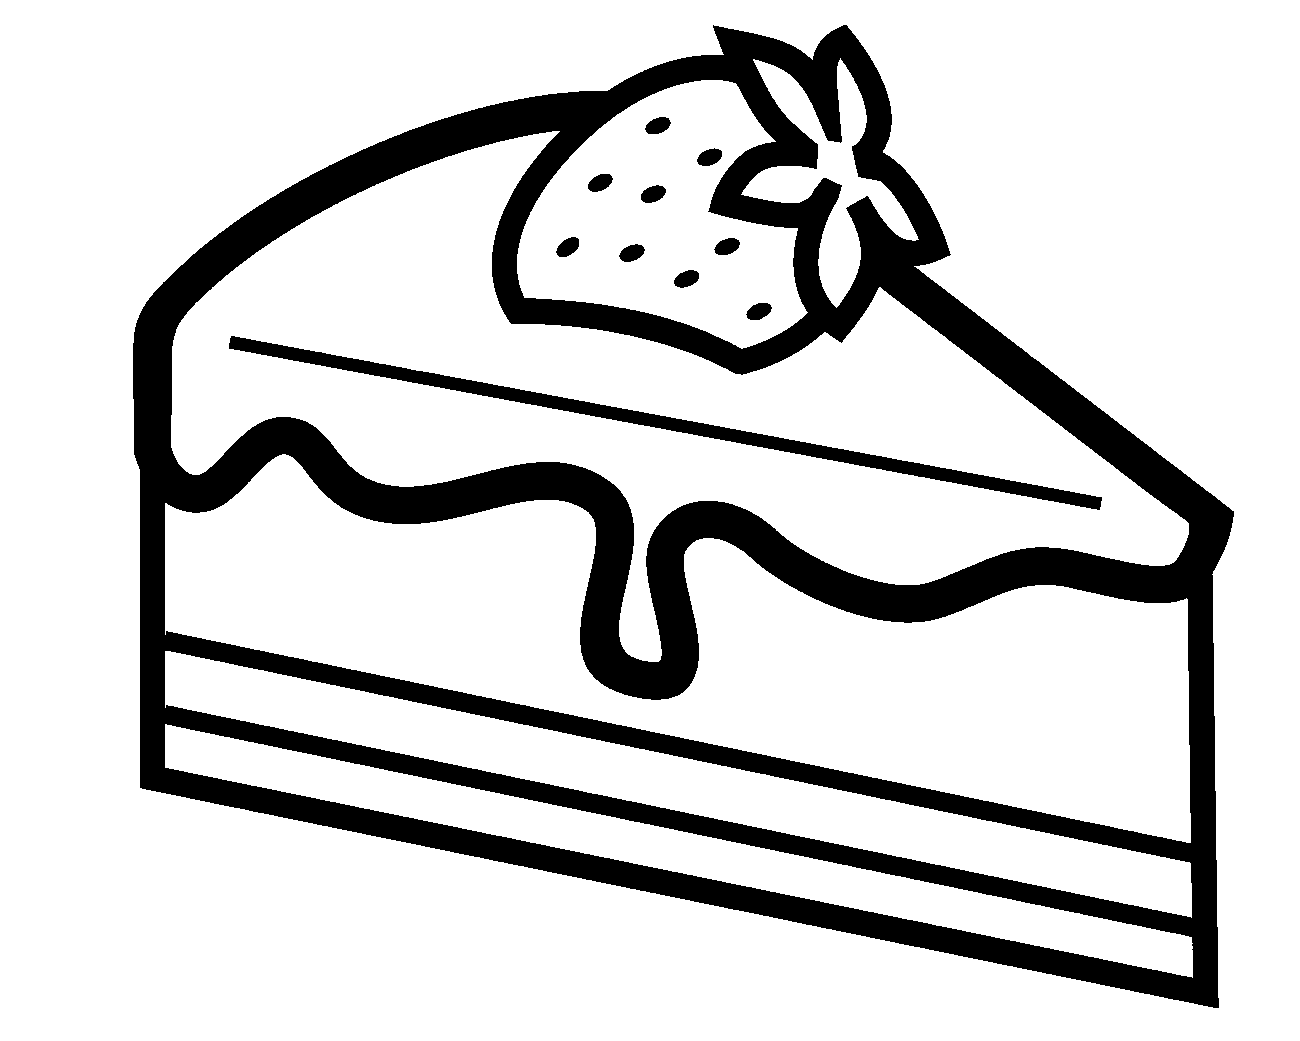
\includegraphics[height=8cm]{06piece_of_cake.png}
	\end{center}
	
	A few mathematicians are celebrating the proof of Fermat's last theorem.
	
	As they are lazy (i.e. proper mathematicians), they want to slice the cake with as few straight cuts as possible.
	
	One claims "amazing, if there was one more person, we would need $5$ cuts, but we only need $4$!\footnote{(this is not factorial $4!=24$, just $4$ with excitement form the speaker)}".
	
	\vspace{1cm}
	
	\begin{center}
		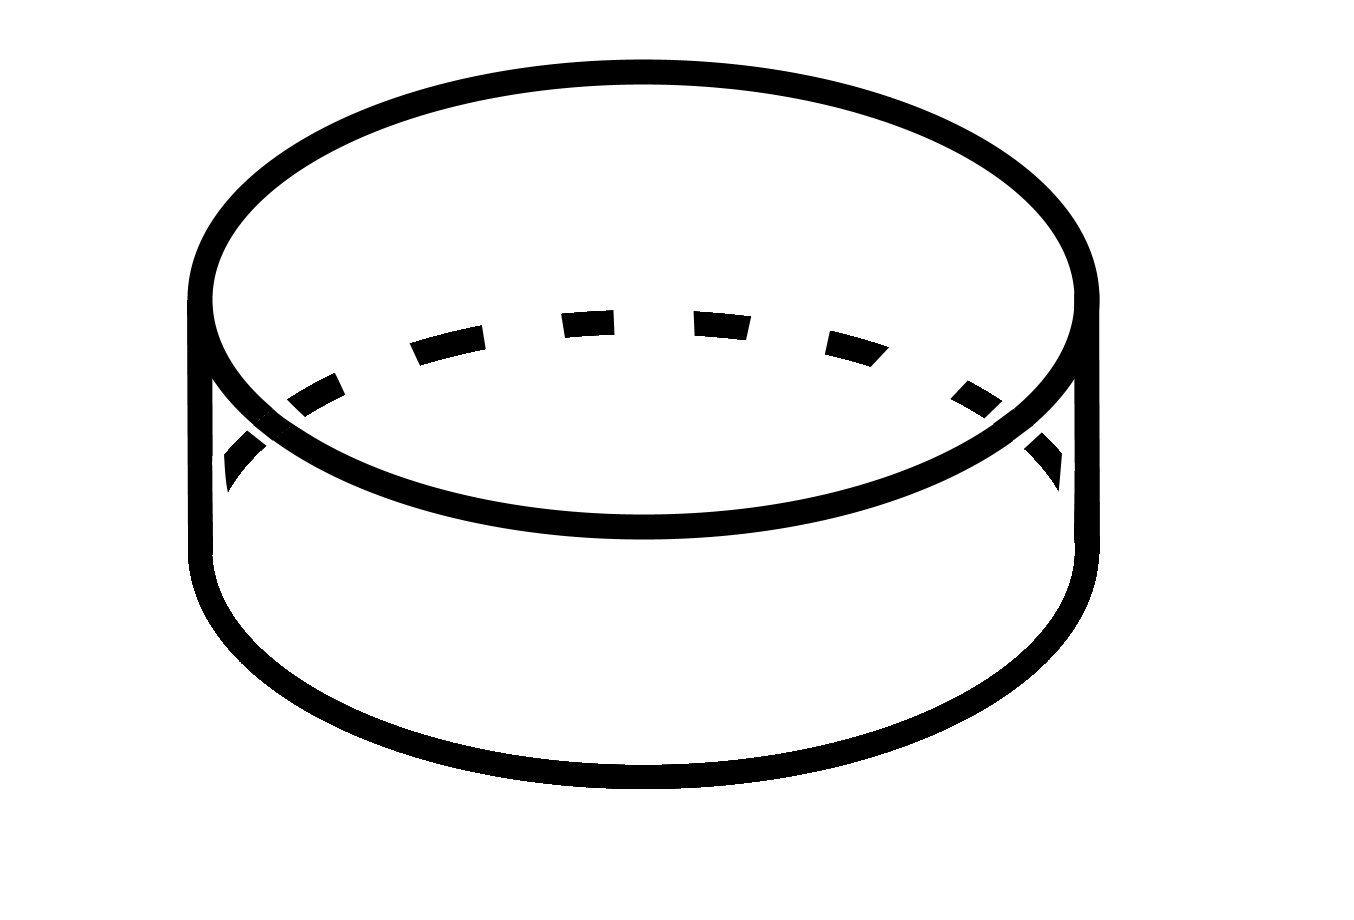
\includegraphics[height=5cm]{06cylinder.png}\\
		\textit{[The cake is considered to be a perfect cylinder, for simplicity.]}
	\end{center}
	
	\vspace{1cm}
	
	\textbf{How many mathematicians are in the room?}
	
\end{document}